%%%%%%%%%%%%%%%%%%%%%%%%%%%%%%%%%%%%%%%%%
% Journal Article
% LaTeX Template
% Version 1.4 (15/5/16)
%
% This template has been downloaded from:
% http://www.LaTeXTemplates.com
%
% Original author:
% Frits Wenneker (http://www.howtotex.com) with extensive modifications by
% Vel (vel@LaTeXTemplates.com)
%
% License:
% CC BY-NC-SA 3.0 (http://creativecommons.org/licenses/by-nc-sa/3.0/)
%
%%%%%%%%%%%%%%%%%%%%%%%%%%%%%%%%%%%%%%%%%

%----------------------------------------------------------------------------------------
%	PACKAGES AND OTHER DOCUMENT CONFIGURATIONS
%----------------------------------------------------------------------------------------

\documentclass[twoside,twocolumn]{article}

\usepackage{blindtext} % Package to generate dummy text throughout this template 

\usepackage[sc]{mathpazo} % Use the Palatino font
\usepackage[T1]{fontenc} % Use 8-bit encoding that has 256 glyphs
\linespread{1.05} % Line spacing - Palatino needs more space between lines
\usepackage{microtype} % Slightly tweak font spacing for aesthetics
\usepackage{amsmath}

\usepackage[english]{babel} % Language hyphenation and typographical rules

\usepackage[hmarginratio=1:1,top=32mm,columnsep=20pt]{geometry} % Document margins
\usepackage[hang, small,labelfont=bf,up,textfont=it,up]{caption} % Custom captions under/above floats in tables or figures
\usepackage{booktabs} % Horizontal rules in tables

\usepackage{lettrine} % The lettrine is the first enlarged letter at the beginning of the text

\usepackage{enumitem} % Customized lists
\setlist[itemize]{noitemsep} % Make itemize lists more compact

\usepackage{abstract} % Allows abstract customization
\renewcommand{\abstractnamefont}{\normalfont\bfseries} % Set the "Abstract" text to bold
\renewcommand{\abstracttextfont}{\normalfont\small\itshape} % Set the abstract itself to small italic text

\usepackage{titlesec} % Allows customization of titles
\renewcommand\thesection{\Roman{section}} % Roman numerals for the sections
\renewcommand\thesubsection{\roman{subsection}} % roman numerals for subsections
\titleformat{\section}[block]{\large\scshape\centering}{\thesection.}{1em}{} % Change the look of the section titles
\titleformat{\subsection}[block]{\large}{\thesubsection.}{1em}{} % Change the look of the section titles

\usepackage{fancyhdr} % Headers and footers
\pagestyle{fancy} % All pages have headers and footers
\fancyhead{} % Blank out the default header
\fancyfoot{} % Blank out the default footer
\fancyhead[C]{Running title $\bullet$ May 2016 $\bullet$ Vol. XXI, No. 1} % Custom header text
\fancyfoot[RO,LE]{\thepage} % Custom footer text

\usepackage{titling} % Customizing the title section

\usepackage{hyperref} % For hyperlinks in the PDF

\usepackage{graphicx} % For figures
% \newcommand{\setrefnumber}{\phantomsection\renewcommand{\@currentlabel}}%

\pagestyle{fancy}
\fancyhf{}
\fancyhead[LE,RO]{}

\usepackage{subcaption}

%----------------------------------------------------------------------------------------
%	TITLE SECTION
%----------------------------------------------------------------------------------------

\setlength{\droptitle}{-4\baselineskip} % Move the title up

\pretitle{\begin{center}\Huge\bfseries} % Article title formatting
\posttitle{\end{center}} % Article title closing formatting
\title{Assessing the Quality of Correction for Physiological Effects, on BOLD signal, by Convolving RVT with RRF} % Article title
\author{%
\textsc{Peter Lauren \& Paul Taylor}\\ % Your name
\normalsize Scientific and Statistical Computing Core \\ NIMH, NIH \\ Bethesda, MD, USA\\ % Your institution
}
\date{\today} % Leave empty to omit a date
\renewcommand{\maketitlehookd}{%
\begin{abstract}
\noindent This paper describes a technique for not only accounting for the effects of respiration on the BOLD signal but also taking into account the temporal dependence of this response.  In particular, respiration has a delayed effect on the BOLD signal and an overshoot/undershoot following the initial respiration induced decrease/increase in the signal.  This is addressed by comvolving the Respiration Volume per Time (RVT) with the Respiratory Response Function (RRF).  This appears to model the BOLD response to respiration significantly more accurately than previous techniques.
\end{abstract}
}

%----------------------------------------------------------------------------------------

\begin{document}

% Print the title
\maketitle
\onecolumn
\tableofcontents
\newpage
\twocolumn

%----------------------------------------------------------------------------------------
%	ARTICLE CONTENTS
%----------------------------------------------------------------------------------------

\section{Introduction}

Functional MRI (fMRI) allows researchers to model neuronal activity at different parts of the brain by analyzing blood oxygen level dependent (BOLD) signals. However blood oxygenation also varies with cardiac and respiratory cycles  \cite{Glover2000}.  Fluctuations in breathing during rest generally occur at similar frequencies (~0.03 Hz) and in similar brain regions as those implicated in resting-state default-mode network (DMN) activity \cite{Wise2004}\cite{Birn2006}. The DMN comprises a set of regions that exhibit low-frequency correlated signals in task-free resting state \cite{Greicius2004} and are collectively down-regulated during a wide range of cognitively demanding tasks \cite{McKiernan2003}. The DMN likely reflects both unconstrained mental activity (e.g. ``mind wandering'') as well as spontaneous neuronal fluctuations, and has been shown to reliably map multiple functional networks in the brain\cite{Birn2012}.  Glover {\em et al.}\cite{Glover2000} present an algorithm for modeling such variation. This corrects the signal based on the phase of the cardiac and respiratory cycle in which each image was acquired.  This removes fluctuations at the respiration and cardiac frequencies and their first harmonics.  This deals with physiological fluctuations (e.g. cardiac) that are of a higher frequency than the rate of image acquisition (determined by the repetition time (TR)\footnote{Whole brain imaging generally requires a TR of at least 2-3 s.}), and it allows for a variation in the cardiac and respiration rate. It does not, however, remove the slower (~0.03 Hz) signal changes induced by breath-to-breath variations in the depth and rate of breathing (i.e. the changes in the envelope of the respiration measurement) \cite{Birn2006}.  Additionally, the TR, required for whole brain imaging, results in aliasing of cardiac and respiratory fluctuations to much lower frequencies which are not removed by a simple low pass filter (<0.1 Hz)\cite{Birn2012}. Since RETROICOR\cite{Glover2000} takes into account the phase of the respiration and cardiac cycle at which each image is acquired, respiration and cardiac induced signal fluctuations can be reduced despite aliasing or variations in cycling rate during the acquisition \cite{Birn2012}.  Additionally, spatial specificity of functional connectivity, has been clearly demonstrated to be influenced by aliased physiological noise\cite{Lowe1998}.  There are, however, additional physiological (cardiac and respiratory-related) fluctuations that are not removed by such techniques. Variations in breathing depth and rate, for example, lead to alterations in arterial CO$_2$ levels.  CO$_2$ is a potent vasodilator, leading to increased blood flow and, consequently, increased BOLD signal\cite{Birn2006}.  Increased arterial CO$_2$ levels activate chemoreceptors that increase subsequent breathing depth and rate. This results in increased CO$_2$ exhalation and a reduction of arterial CO$_2$. Studies have shown that fluctuations of arterial CO$_2$ (as measured by a person's end-tidal CO$_2$) vary with a cycle of about 0.03 Hz\cite{Modarreszadeh1994}.  Variability in heart rate is correlated with MRI signal changes throughout gray matter\cite{Chang2009}.  Furthermore, cerebral blood vessels exhibit vasomotion, a spontaneous low frequency (~0.1 Hz) oscillation in vascular tone and blood flow\cite{Hudetz1998}.  A study by Vogt et al. also showed that RETROICOR resulted in a significant reduction in time course variance and increase in the detection of activation to a painful stimulus\cite{Vogt2011}.  However, another study\cite{Jo2010} determined that averaged over gray matter, cardiac and respiratory regressors modeled in RETROICOR account for a small amount of time course variance (R$^2$<0.05), but that this improvement was offset by the loss of degrees of freedom. 

Changes in the respiration volume per time (RVT), reflect changes in the envelope of the respiration changes as well as the rate of breathing \cite{Birn2006}. Changes in the subject’s breathing rate or depth, such as a breath-hold challenge, can cause significant MRI signal changes \cite{Birn1993}.  Even subtle variations in breathing depth and rate that occur naturally during rest can result in significant signal changes \cite{Wise2004}\cite{Birn2006}.  Respiratory Volume per Time (RVT) is believed to capture breathing-induced changes in arterial CO$_2$, which is a cerebral vasodilator \cite{Chang2009}.  While the effect varies throughout the brain, the fMRI signal tends to be negatively correlated with the breathing depth \cite{Birn2012}. Temporal changes in respiration volume per time (RVT) is significantly correlated with MRI signal variations \cite{Birn2006}.  Separate studies have found that spontaneous fluctuations in end-tidal CO$_2$ (PETCO$_2$) are correlated with BOLD signal time series \cite{Chang2009}. However, respiration related signal changes appear to be slower than neuronally-induced BOLD signal changes \cite{Birn1993}. Also, RVT time course is dominated by low frequency changes. Deconvolution therefore amplifies the high frequencies, resulting in an extremely noisy estimate of the impulse response \cite{Birn2006}. Additionally, a number of brain regions are activated in association with voluntary changes in breathing\cite{McKay2003}.

Changes in arterial CO$_2$ do not occur immediately after a change in the breathing volume or rate, but may take several seconds to develop \cite{VandenAardweg2002}. Additionally, signal changes induced by an administration of CO$_2$ have been observed to result in relatively slow signal changes, with a time constant of approximately 45 seconds and a delay of approximately 6 seconds \cite{Poulin1996}\cite{Corfield2001}.  MR signal response to breath-holding has often shown a strong bimodal response, with an early signal decrease followed by a later overshoot, particularly when the breath hold is performed after inspiration \cite{Birn2008}.  A decrease in the breathing depth or rate results in an initial decrease in signal followed by a strong overshoot, while an increase in the breathing depth or rate results in an initial overshoot with a later decrease \cite{Birn2008}.  Removing the variance in the MRI signal induced by respiration changes requires a function that is not only roughly correlated with the response, but one that matches the precise temporal shape of the induced signal change. A sudden change in breathing rate or depth, for example, results in a relatively slow flow and oxygenation change \cite{Birn2008}.   These delayed BOLD responses to respiration necessitate a transfer function between respiration changes and MRI signal changes \cite{Birn2008}.

\section{Functional Connectivity}

Functional connectivity typically refers to a high level of temporal correlation among spatially distinct locations within the brain.  Birn \cite{Birn2012} estimated functional connectivity among different brain regions from MRI data by computing the temporal correlation of low frequency (<0.1 Hz) fluctuations in the MRI signal.  These fluctuations occurred even when the subject was ``at rest''.  Correlated signal fluctuations occurred at low temporal frequencies (<0.1 Hz).  Biswal {\em et al.}\cite{Biswal1995} found that signal fluctuations in the left and right primary motor areas were significantly correlated even when the subject was not performing any motor task.  These correlated signal fluctuations occurred at low temporal frequencies (<0.1 Hz)\cite{Birn2012}.

Birn\cite{Birn2012} gave a number of reasons for seeing spatially separated functional networks as neuronal rather than artifactual.
\begin{itemize}
	\item Correlations are observed between functionally related brain areas. 
	\item Correlated signal fluctuations in functionally related brain regions are not due to cardiac pulsations and respiration but instead occur at much lower temporal frequencies\cite{Biswal1995}.
	\item These fluctuations have similar characteristics as neuronally-induced BOLD responses (e.g. TE dependence, attenuation of the response during hypercapnia)\cite{Biswal1997}.  If anything, removing cardiac and respiratory-related fluctuations made the map of connectivity to the posterior cingulate look more like the map of areas deactivated during tasks\cite{Birn2012}.  Correlated fluctuations in the DMN remain (and in fact increase) even when the arterial CO$_2$ levels, as measured by end-tidal CO$_2$, are held more constant\cite{Madjar2011}.
	\item Correlations are observed in multiple distinct functional brain networks\cite{Beckmann2005}.  This does not appear to be related to similarities in vascular structure\cite{Birn2012}.
	\item Studies have shown that a disruption in structural connectivity leads to a reduction in resting-state functional connectivity.
	\item A resting-state functional connectivity study by Krienen and Buckner showed that the left cerebellum was more strongly coupled with the right primary motor cortex, and conversely that the right cerebellum was more strongly coupled with the left motor cortex.
	\item Correlated fluctuations in neuronal activity have been demonstrated with other modalities, such as EEG\cite{Laufs2003}.
\end{itemize}

\section{Respiratory Response Function}

The Respiratory Response Function (RRF) models the average BOLD response to a single deep breath.  It has the following form.
\begin{eqnarray}
	RRF(t) = 0.6t^{2.1}e^{\frac{-t}{1.6}}-0.0023t^{3.54}e^{\frac{-t}{4.25}}
\end{eqnarray}

\begin{figure}[htb]
	\begin{center}
		\includegraphics[height=2.5in,width=3in,angle=0]{/home/peterlauren/retroicor/RVTRRF/RRF.pdf}
		\caption{RRF in response to a single deep breath.}
		\label{fig:RRF}
	\end{center}
\end{figure}

This is shown, for the first 50 seconds from the start of the breath, in figure \ref{fig:RRF}.  Birn {\em et al} found that the correlation coefficient between the idealized RRF and the averaged and deconvolved response to a single deep breath was 0.935. They also found that the effects of cued breath changes (breath holding, rate changes and depth changes) on the BOLD signal, were accurately modeled by RVT convolved with RRF (RVTRRF). The majority of the signal change resulted from the undershoot in the RRF, leading to the pronounced signal overshoot in response to breath-holding, and the signal decrease in response to increases in respiration depth or rate. These respiration-induced changes were generally slower than neuronally-induced BOLD fMRI signal changes, and were therefore not as accurately modeled with the gamma-variate or canonical Statistical Parametric Mapping (SPM) hemodynamic response function.  Signal changes induced by variations in breathing during rest appeared to be slightly faster, and were not modeled as well using either RFF or the hemodynamic response functions typically used to analyze neuronally-induced BOLD changes. Allowing a variation in the latency of the respiration response resulted in a significantly better fit, particularly for the gamma-variate response function, canonical SPM response function, and delta function IRF (i.e. simply a shifted RVT or ideal stimulus timing) \cite{Birn2008}.  There is a wide range of optimal latencies across voxels, approximately $\pm 5$ s relative to the average latency which is 5.4s\cite{Birn2012}.  The optimal latency for RRF is closer to zero. The peak of this histogram is slightly less than zero for RRF, indicating that the estimated RRF may be too slow for several voxels \cite{Birn2008}.  For most voxels, the optimal latency, for RVTRRF at rest, is about -8 s.  The latency and temporal evolution of the average respiration induced signal change was found to vary across the brain by several seconds \cite{Birn2008}.  The variation in latency is driven by a difference in the width of the response, rather than a large difference in the onset time \cite{Birn2008}. 
 
\subsection{Subsequent Analysis}

Chang \& Glover \cite{Chang2009} confirm the advantages of convolving RVT with the RRF.  In particular, convolving with RRF yields an optimal linear mapping of RVT to fMRI time series \cite{Chang2009}.
 
RVT (particularly when convolved with a particular impulse response, the “respiration response function”) is highly correlated with PETCO$_2$

Respiration changes the BOLD signal by altering the levels of CO$_2$, a potent vasodilator.  Vasodilation leads to increased cerebral flow which effects the BOLD signal.  The partial pressure of arterial CO$_2$ (PaCO$_2$) is a function of ventilation, which is defined as the product of the depth and rate of respiration \cite{Birn1993}.  Increased CO$_2$ increases cerebral blood flow (CBF), leading to decreased concentrations of deoxyhemoglobin and thus an increase in $T2^*$ (BOLD contrast) with a corresponding increase in BOLD signal.  Decreased CO$_2$ has the opposite effects.  RVT may account for variance in the BOLD signal beyond that which can be explained by CO$_2$ levels \cite{Chang2009}.

Chang \& Glover \cite{Chang2009} colvolved RVT with RRF to obtain the result, RVTRRF.  Among their findings:
\begin{itemize}
	\item The cross-correlation between PETCO$_2$ and RVTRRF was positive ($\bar{Z} = 18.3, SD=2.55$), having a single clear maximum, and was of significantly greater magnitude than cross-correlations between PETCO$_2$ and RVT ($p < 0.05$, paired t-test).
	\item PETCO$_2$ preceded RVTRRF by an average of 11.14 s (SD=1.07 s).
	\item RVTRRF represents the modeled BOLD signal output to variations in breathing (as measured with a respiration belt), and its high correlation with the (time-delayed) PETCO$_2$
	\item Performing a convolution between RVT and the RRF acts primarily to negate and smooth the RVT signal.
	\item Correlations between PETCO$_2$ and PETO$_2$ were strongly negative ($\bar{Z} = -22.3, SD=3.94$).
	\item In some subjects and voxels, RVTRRF showed a stronger relationship with the BOLD signal than PETCO$_2$, while in others the opposite was true.
	\item Including both PETCO$_2$ and RVTRRF in the model explained more variance than either signal individually.
	\item RVTRRF was found to explain significantly greater variance than RVT in an average of 26\% of voxels, whereas RVT explained significantly greater variance than RVTRRF in an average of 4.4\% of voxels.
	\item The average time delay between PETCO$_2$ and BOLD signal change was $10 \pm 1.6$ s.  Time delays between RVTRRF and the BOLD signal were centered near 0 ($0.06 \pm 2.8$ s)
	\item The cerebellum exhibited a consistently high latency.
	\item PETCO$_2$ has the potential for being “noisier” than RVTRRF
	\item A simple time-shift of PETCO$_2$ time series was found to predict a significant component of the BOLD signal time series.
	\item RVT was negatively correlated with PETCO$_2$ after a time delay of approximately 5 s (1–2 breaths).
	\item Convolving RVT with the RRF impulse response enhanced the cross-correlation with PETCO$_2$.
\end{itemize}

\subsection{Application}

Figure \ref{FigRVTRRF} shows an example of RVT being convolved with RRF.  When RRF is convolved with the original RVT, the resulting RVTRRF shows {\em edge effects}.  To remove these effects, RVT is {\em floated} by subtracting the mean of RVT rom the RVT vector and the result is convolved the RRF to obtain the modified RVTRRF.  That is
\begin{eqnarray}
	RVTRRF = RRF * (RVT-\hat{RVT})
\label{floatedRVTRRF}
\end{eqnarray}

As one can see (figure \ref{fig:sfig3}), this removes the edge effects and pushes RVTRRF towards the x-axis.

\begin{figure}
	\begin{subfigure}{.5\textwidth}
		\centering
		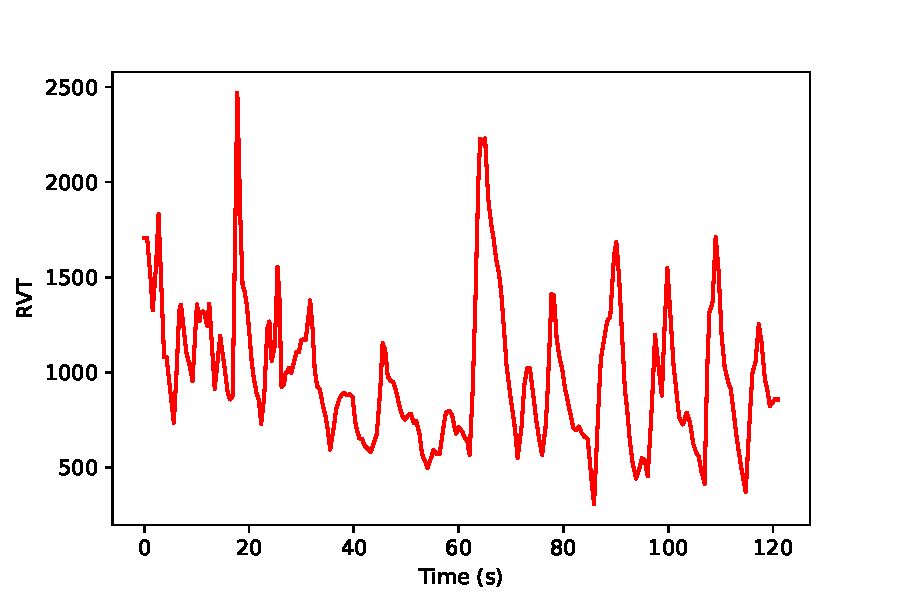
\includegraphics[width=.8\linewidth]{/home/peterlauren/retroicor/RVTRRF/FigRVT.pdf}
		\caption{RVT}
		\label{fig:sfig1}
	\end{subfigure}%
	\\
	\begin{subfigure}{.5\textwidth}
		\centering
		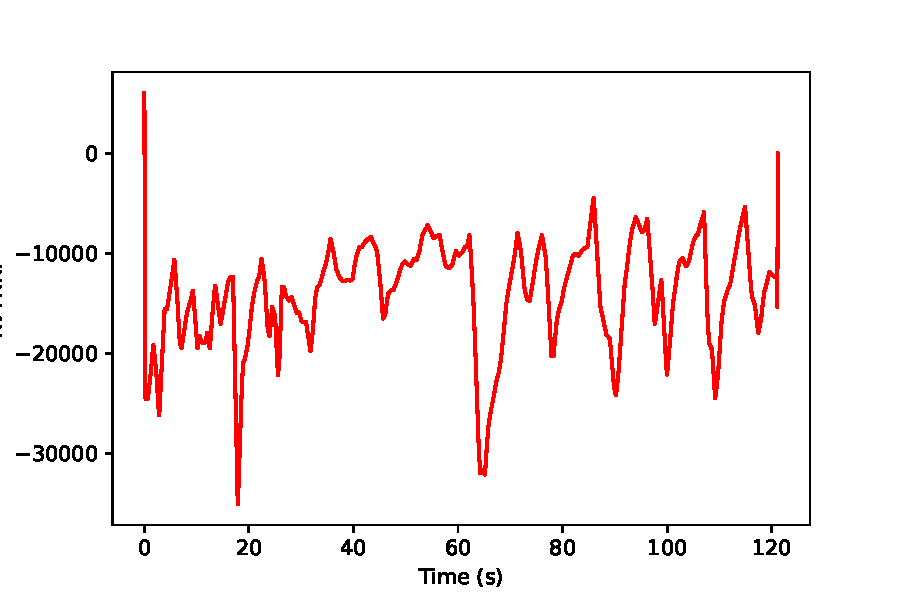
\includegraphics[width=.8\linewidth]{/home/peterlauren/retroicor/RVTRRF/FigRVTRRF.pdf}
		\caption{RVTRRF}
		\label{fig:sfig2}
	\end{subfigure}
	\\
	\begin{subfigure}{.5\textwidth}
		\centering
		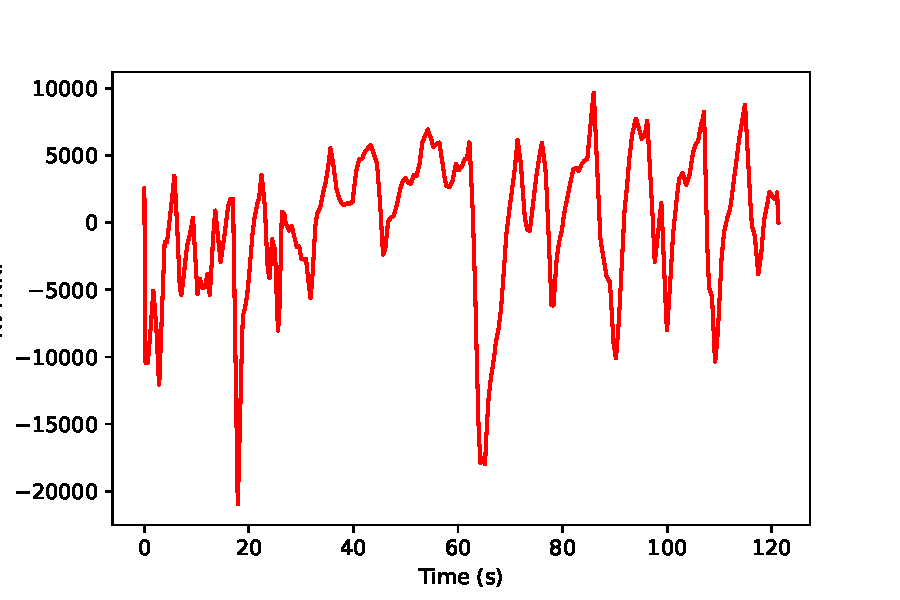
\includegraphics[width=.8\linewidth]{/home/peterlauren/retroicor/RVTRRF/FigFloatedRVTRRF.pdf}
		\caption{RVTRRF with Floated RRF}
		\label{fig:sfig3}
	\end{subfigure}
	\caption{Plots of (\ref{fig:sfig1}) RVT,  (\ref{fig:sfig2}) corresponding RVTRRF and (\ref{fig:sfig3}) RVTRRF with the edge effects removed by {\em floating} the RVT vector.}
	\label{FigRVTRRF}
\end{figure}

\section{Combining Cardiac and Respiratory Response Functions}

A study by Dagli {\em et al.}\cite{Dagli1999} found that significant cardiac fluctuations were found on average in $27.5 \pm 8.0\%$ of the brain voxels. Removing these fluctuations resulted in a variance reduction of roughly 10-40\%, depending on the region being investigated.  Chang {\em et al}\cite{Chang2009b} deconvolved the resting state fMRI with the combined effects of respiration variation (RV) and heart rate (HR). RV was based on computing the standard deviation of the respiratory waveform on a sliding window of 3 TRs centered at each desired TR sampling point. Specifically, the value of the RV time series assigned to the kth TR was computed by taking the standard deviation of the raw respiratory waveform over the $3 \times TR$ time interval.  The main advantage they identified for this, over RVT, is that it obviates accurate peak and trough detection.  They concede that RVT considers a shorter interval (breath-to-breath, which tends to be 3-4 s) and accounts more explicitly for variations in breathing rate by normalizing the depth by the breath-to-breath time interval. While simpler to compute than RVT (no peak detection in the respiration waveform is required), the use of a fixed-length sliding window rather than breath-to-breath intervals is more difficult to interpret due to its complex dependence on the depth, frequency, and phase of respiratory cycle within each window.   This would argue in favor of using RVT, instead of RV, if peaks and troughs can be accurately determined.

The HR(k) time series was computed by averaging the time differences between pairs of adjacent ECG triggers contained in the $3 \times TR$ window and dividing the result into 60 to convert it to units of beats per minute.  The time series of a voxel, $y$, is modeled as the sum of RV convolved with an unknown RV filter, $h_r$, and HR convolved with an unknown HR filter, $h_h$, plus a noise term, $\epsilon$:
\begin{eqnarray}
	y = X_rh_r + X_hh_h + \epsilon
	\label{RVHR}
\end{eqnarray}
where $h_r \sim N(0,K_r)$\footnote{N(a,b) denotes a normal distribution with mean, $a$ and variance $b$.}, $h_h \sim N(0,K_h)$, and $\epsilon \sim N(0,\sigma_{\epsilon}^{2}I)$ is usually set to the sample variance of the $i^{th}$ voxel time series. $X_r$ and $X_h$ refer to the convolution matrices defined by RV and HR, respectively.  $\sigma_{\epsilon}^2$ is the variance of the noise.  The covariance matrices $K_r$ and $K_h$ describe the degree of correlation between points in $h_r$ and $h_h$ as a function of their distance, and are defined here as
\begin{eqnarray}
	[K_r]_{ij}=[K_h]_{ij}=\sigma_f^2\exp\left(-\frac{(i-j)^2}{2l^2}\right)
\end{eqnarray}
$l$ (typically 2) governs the degree of smoothness.   Larger $l$ produces more slowly varying filters.  The kernel variance, $\sigma_f^2$ (typically 1), regulates the distance from which values of $h$ depart from its mean.  The model, defined by equation \ref{RVHR} is called the RVHR model.  $h_r$ and $h_h$ begin and end at 0 and have typical durations of 30 s.

 They observed that a convolution model including RV and HR can explain significantly more variance in gray matter BOLD signal than a model that includes RV alone.  They also observed that modeling out RV and HR can significantly alter functional connectivity maps of the DMN.  HR appears to be negatively correlated with the BOLD signal time series at time lags ranging from 6–12 s, and positively correlated at time lags of 30–42 s \cite{Shmueli2007}.
 
 RV and HR were only mildly correlated.  Regions correlated with HR tended to comprise gray matter, and were often disjoint from regions correlated with RV.  For all but one, out of 10 subjects, the RVHR model explained significant variance over a greater spatial extent than the RV and RRF models, and accounted for a larger mean percentage of the signal variance.  The relative performance of RRF and RV likely depends on the quality of the peak and trough detections but this needs to be tested.  Correcting for RV and HR tended to decrease the overall spatial {\em extent} of DMN connectivity.  The reductions were roughly 1.0\% of voxels after the RRF model correction, 5.6\% after the RV model correction, and 7.6\% after the RVHR model correction.  RVHR appears to impact DMN connectivity much more than does RETROICOR and preprocessing with RETROICOR (prior to applying RVHR) does not appear to make a significant difference compared with applying RVHR alone (p>0.5) \cite{Chang2009b}.  regions in which the HR component had a significant effect were often disjoint from regions in which the effects of RV (and RRF) were significant, indicating differential contributions of HR and RV effects over space \cite{Chang2009b}.  Deconvolution of the HR response revealed that the majority of responsive voxels exhibited a peak at around 4 s and an undershoot of approximately equal magnitude at around 12 s. These features were remarkably consistent across subjects and anatomical regions \cite{Chang2009b}.
 
 Chang {\em et al}\cite{Chang2009b} also formulated a {\em Cardiac Response Function} (CRF) given by equation \ref{CRF} and shown in figure \ref{fig:CRF}.  This was convolved with the HR time series.
\begin{eqnarray}
	CRF(t)=0.6t^{2.7}e^{\frac{-t}{1.6}}-16\frac{1}{\sqrt{2\pi(9)}}\exp\left(-\frac{(t-12)^2}{18}\right)
	\label{CRF}
\end{eqnarray}

\begin{figure}[htb]
	\begin{center}
		\includegraphics[height=2.5in,width=3in,angle=0]{/home/peterlauren/retroicor/RVTRRF/CRF.pdf}
		\caption{CRF response function which is convolved with HR(t).}
		\label{fig:CRF}
	\end{center}
\end{figure}

Cardiac pulsation also results in brain tissue movement and inflow effects leading to correlated signal fluctuations primarily in and near large blood vessels\cite{Dagli1999}.

\section{End Tidal CO$_2$ Measurements}

Including measures of end-tidal CO$_2$ explains noise not accounted for by RETROICOR coefficients and RVT(RRF)\cite{Birn2012}.

\section{Floating the Brain Volume}

Regressing out the average signal over the whole brain has been shown to result in the regions significantly correlated with the posterior cingulate to became more focal in space and matched more closely with the areas that were deactivated during the lexical task \cite{Birn2012}.  Some investigators have started to use the average signals over the white matter and CSF as nuisance regressors\cite{Birn2012}. 

\section{Connectivity Exaggeration due to Nuisance Factors}

Preprocessing the image data using AFNI\cite{Cox1996}, Hallquist {\em et al}\cite{Hallquist2013} observed how head motion, and other nuisance factors exaggerated resting-state functional connectivity fMRI (RS-fcMRI) estimates which is the dominant method for characterizing the human functional connectome.  The most common unfiltered nuisance regressors, they encountered, were motion parameters (73\%).  They considered three methods for applying bandpass filtering and nuisance regression.
\begin{itemize}
	\item Bandpass filtering (0.009-0.08 Hz) followed by nuisance regression (BpReg).  With this approach, nuisance regressors are not bandpass filtered.
	\item Regression followed by bandpass filtering (RegBp).  Nuisance regression is performed on preprocessed functional data, and the residuals from the regression model are subsequently bandpass filtered.
	\item Simultaneous bandpass filtering and regression (Simult).  This approach is accomplished by the 3dBandpass program, in AFNI \cite{Cox1996}, using the -ort option for nuisance regression.
\end{itemize}

Noise sources typically include power at frequencies in the stop band (i.e., the frequencies to be suppressed), leading to statistical dependence between the spectral filter and nuisance regressors.  Thus, the manner in which bandpass filtering and nuisance regression are applied to RS-fcMRI data may affect the quality of noise in RS-fcMRI data, as well as estimates of functional connectivity.  Hallquist {\em et al}\cite{Hallquist2013} demonstrated that nuisance regression model is misspecified in the frequency domain when the fMRI time series are bandpass filtered but one or more regressors are unfiltered, resulting in the reintroduction of temporally synchronous nuisance-related variation into frequencies previously suppressed by the bandpass filter, as well as suboptimal correction for nuisance signals in the frequencies of interest. By contrast, there was no frequency mismatch in the nuisance regression for bandpass filtering after regression (RegBp) and simultaneous filtering (Simult), so these approaches do not suffer from that flaw.

Greater head motion has been associated with increased estimates of short-range connectivity and potentially suppressed estimates of long-range connectivity \cite{Hallquist2013}.  Motion-related fluctuations in the overall BOLD signal contaminates RS-fcMRI time series despite bandpass filtering and nuisance regression \cite{Power2012}. 

Hallquist {\em et al}\cite{Hallquist2013} used heartbeat signals to create RETROICOR regressors for each axial slice that represented cardiac-related fluctuations in the fMRI time series at the time of image acquisition.  However, they did not use the RETROICOR regression approach to mitigate cardiac artifacts. Rather, RETROICOR data were used to characterize whether the strength of cardiac artifacts in RS-fcMRI time series differed among preprocessing approaches. 

Hallquist {\em et al}\cite{Hallquist2013} also found that BpReg reintroduces nuisance variation into stop-band frequencies and poorly attenuates nuisance variation in the pass-band. They found that regression of a bandpass-filtered fMRI time series on full-spectrum nuisance regressors (BpReg) results in considerable distortion of the fMRI signal by bandpass filtering the fMRI time series, but not the noise signals.  The regression model is misspecified in the frequency domain such that nuisance variability is systematically under-controlled. This occurs because standard regression methods optimize the fit of two time series across all frequencies present in both signals \cite{Engle1974}, yet the fluctuations in the stopband frequencies have been suppressed from the fMRI signals but not the nuisance regressors. Consequently, the fit of the regression (and the variance explained) is shifted toward zero. Moreover, the misspecified regression under the BpReg approach reintroduces temporally synchronous nuisance fluctuations into RS-fcMRI time series at frequencies previously suppressed by the bandpass filter. \cite{Hallquist2013}.  Residual fluctuations in the global BOLD signal attributable to head motion were largely eliminated by the Simult approach, whereas weak residual motion-related fluctuations were evident for RegBp.  RegBp regression optimizes a single parameter estimate that captures the association of an fMRI signal and a given nuisance signal across all observed frequencies, yet the fMRI–nuisance relationship is often heterogeneous across the spectrum.   variability in connectivity estimates attributable to head motion was 94\% lower for Simult than for BpReg \cite{Hallquist2013}.

From \cite{Hallquist2013}, the periodic symbol, $M$, representing participant motion during the 200 s fMRI acquisition, composed of sinusoidal frequencies at 0.06, 0.2, 0.3, and 0.4 Hz, can be given by equation \ref{HallquistMotion}.
\begin{eqnarray}
	\begin{split}
	M=\sum_{t=1}^n\cos\left(2\pi t\frac{12}{n}\right)+\cos\left(2\pi t\frac{40}{n}\right)+  
	\\
	\sin\left(2\pi t\frac{60}{n}\right)+\cos\left(2\pi t\frac{80}{n}\right)
	\end{split}
\label{HallquistMotion}
\end{eqnarray}

They subsequently model the corrupted signal, $C$, given the original fMRI signal, $X$, using equation \ref{motionCorruption}.
\begin{eqnarray}
	C=X+0.8M_{0.06 Hz}+0.6M_{0.2 Hz}+
	\\ 0.4M_{0.3 Hz}+0.2M_{0.4 Hz}
\label{motionCorruption}
\end{eqnarray}

since lower-frequency components were associated with larger signal fluctuations. The relationship between the dependent variable, $C$, and the independent variable, $M$, varies across the spectrum\cite{Engle1974}. Variance explained by nuisance regression for the bandpass–regress approach is approximately half that explained under the Simult approach\cite{Hallquist2013}.  Nuisance regression reintroduces high-frequency variability into the MR signal previously suppressed by the bandpass filter, effectively ``leaking'' spectral power precisely at the frequencies present in the original motion signal, $M$\cite{Hallquist2013}.  In time series regression, parameter estimates tend to be dominated by the strongest frequency components present in the series because these are associated with the greatest variability \cite{Engle1974}.  BpReg under-corrects for nuisance variation in the frequencies of interest (0.009-0.08 Hz) and introduces temporally synchronous nuisance variation into the MR signal at frequencies that were previously bandpass filtered. By contrast, the RegBp and Simult filtering approaches were not associated with the introduction of nuisance artifacts\cite{Hallquist2013}.  Simult performs as well as or better than RegBp for removing nuisance variation within passband frequencies.  Simult outperforms RegBp because it optimizes its fit within the passband frequencies\cite{Hallquist2013}.  BpReg did a poor job of removing nuisance variability relative to Simult.  Within the passband, spectral power was significantly lower for Simult than BpReg.  All three approaches, however, had significantly less power in the passband frequencies relative to Raw.  High-frequency covariation between nuisance signals and MR time series for BpReg was significantly higher than RegBp and Simult.  There was no significant difference between RegBp and Simult in the high-frequency stopband.  In the low-frequency stopband (<0.009 Hz), MR-nuisance covariation was significantly higher for BpReg than for Simult and RegBp (z = 2.22, p = .05), whereas Simult and RegBp did not differ from each other.  Cross-spectral power was significantly lower for Simult than BpReg.  Nuisance regressors and RS-fcMRI time series were also much more temporally synchronous for the BpReg approach than the Simult and RegBp approaches.  Bandpass filtering and nuisance regression (using BpReg) did not eliminate large-amplitude changes in the average BOLD signal across the brain that result from head motion\cite{Power2012}.  Bandpass filtering of the fMRI time series without nuisance regression attenuated motion-related BOLD fluctuation to some degree, but also appeared to spread the deleterious effects of motion in time \cite{Hallquist2013}.  Large-amplitude BOLD signal fluctuations across the brain, often in opposite directions, were evident for BpReg at the time of large movements, whereas the RegBp and Simult BOLD signal was much smoother across the brain.  Simult better attenuates nuisance variability within the frequencies of interest in resting-state fMRI data.  Head motion was associated with larger functional connectivity estimates for short-range connections.  For Simult, the motion–connectivity association was generally weak.  The absolute motion–connectivity association was significantly greater for BpReg than Simult.  Motion scrubbing significantly attenuated the head motion–connectivity association for the BpReg approach. The effects of scrubbing for BpReg differed as a function of interregional distance.  Scrubbing the Simult data magnified the negative motion–connectivity association for connections from 100 to 120 mm apart.  The effects of scrubbing depended on the interregional distance.  The average absolute motion–connectivity association for the unscrubbed Simult data was much lower than the scrubbed BpReg data regardless of interregional distance. BpReg approach led to an average motion–connectivity association over 50\% stronger than for Simult. Motion scrubbing attenuated this effect modestly for both BpReg and Simult, particularly for short-range connections. For the Simult approach, scrubbing attenuated the motion–connectivity association for short-range functional connections, but it also increased this association for long-range connections.  Motion–connectivity association was highest for short-range connections.   The magnitude of BpReg–Simult connectivity differences were negatively associated with distance from the center of the brain.  Roughly one-quarter of the data were discarded by motion scrubbing.  Simult did not completely eliminate distance-dependent differences in the association between head motion and functional connectivity estimates \cite{Hallquist2013}.

The average amplitude of cardiac artifacts in the RS-fMRI data, based on the RETROICOR method\cite{Glover2000}, was significantly correlated with the average connectivity difference between BpReg and Simult.  Cardiac artifacts were significantly associated with greater inflation of functional connectivity estimates under the BpReg approach relative to Simult \cite{Hallquist2013}.

\subsection{DVARS}

DVAS is the average root mean square variance across voxels of the temporal derivative of the fMRI time series\cite{Power2012}.  For BpReg, DVARS was significantly higher for contaminated than uncontaminated volumes\cite{Hallquist2013}.  For Simult, DVARS was slightly lower for contaminated frames than for uncontaminated frames.  Simult approach best controlled motion-related BOLD fluctuation.

\section{Bayesian Information Criterion (BIC)}

The goal of higher spatial resolution has spurred the exploration of multi-shot 3D acquisition strategies which are more sensitive to physiological fluctuations as errors between the k-space segments result in strong temporal fluctuations in image space\cite{Tijssen2014}.  RetroICor inherently assumes that each image is acquired instantaneously. Although this assumption is justified for single-shot acquisitions, where the entire slice is acquired in a few tens of milliseconds, it is not for 3D imaging methods, in which the data of a single volume are typically acquired over a period of seconds \cite{Tijssen2014}.  Furthermore, not all regressors optimized for GRE-EPI may be as efficient for 3D FMRI data, since the BOLD-related physiological fluctuations are likely to be different due to the typically shorter repetition time (TR) and echo time (TE) as well as the segmented nature of the acquisition \cite{Tijssen2014}.

According to Tijssen {\em et al}\cite{Tijssen2014}, the loss in degrees of freedom (DOF), due to inclusion of a large number of regressors or correlations of the confound regressor with the regressor of interest, can actually degrade statistical significance
They found that trimming regressors, for 3D acquisitions, to an optimal orthogonal set achieves optimal balance between variance reduction and potential over-fitting.  From \cite{Kass1993}, BIC is given by equation \ref{BIC}
\begin{eqnarray}
	BIC = N\ln\left(\frac{RSS}{N}\right)+k\ln(N)
	\label{BIC}
\end{eqnarray}

where $N$ is the number of time point samples, $k$ is the number of regressors and $RSS$ is the residual sum of squares.  The BIC is used to compare different models, particularly models with a different number of parameters/regressors, with low BIC indicating a favorable model. BIC selection favors models that explain a large portion of the variance, which is weighted against a penalty for the total number of regressors\cite{Tijssen2014}.  The optimal model varies among the various acquisitions types tested.

The selection procedure aims to find the optimal set of regressors iteratively by expanding the model to encapsulate one additional regressor at a time and comparing the resulting BIC score. If the BIC is smaller, it is included in the ``optimal'' set; otherwise, the penultimate model (without the most recently-added regressor) is considered to be optimal. The order in which the regressors are added to the model is determined based on the performance of each regressor when tested individually. The procedure is as follows \cite{Tijssen2014}.
\begin{enumerate}
	\item Regressions are run using each of the candidate regressors as a single regressor. Temporal variance maps are calculated for each of the data sets.
	\item The regressors are sorted based on how much variance each regressor explains within a given region of interest (ROI). The variance reduction is assessed based on the mean variance across the part of the brain of interest.  For Tijssen2014 {\em et al}\cite{Tijssen2014},  this was the brainstem.
	\item An optimal regressor set is created iteratively by adding one regressor at a time in the order determined in step 2. After each model expansion step the BIC value is calculated using the mean RSS within the brainstem ROI. The set of regressors with the lowest BIC is taken as the optimal model for the correction.
\end{enumerate}

Tijssen {\em et al}\cite{Tijssen2014}  found that, while k-space corrections are more robust when performed on real/imaginary than magnitude/phase data, k-space corrections do not outperform image-space corrections,

\section{Discussion}

The current procedure is to first apply the Glover\cite{Glover2000} algorithm, using retroicor or physio\_calc.  This is followed by correction using RVTRFF.  RRF describes the {\em average} respiration induced response function across the brain.  Future research should try to resolve spatial variability, in the BOLD response to respiration, across the brain.  Additionally, RRF is based on a deep breath where there is an initial increase in signal followed by a strong undershoot.  It does not account for cued breath holding or decrease in the breathing depth or rate where there is an initial decrease in signal followed by a strong overshoot.  Perhaps another model should be developed for this.
 

%------------------------------------------------


%----------------------------------------------------------------------------------------
%	REFERENCE LIST
%----------------------------------------------------------------------------------------

\begin{thebibliography}{99} % Bibliography - this is intentionally simple in this template

	\bibitem{Glover2000} Glover GH, Li T-Q \& Ress D (2000). ``Image-Based Method for Retrospective Correction of Physiological Motion Effects in fMRI: RETROICOR''. {\em Magnetic Resonance in Medicine} 44:162–167 (2000)
	
	\bibitem{Birn2012} Birn, RM, (2012), ``The role of physiological noise in resting-state functional connectivity'', {\em NeuroImage} 62:864–870
	
	\bibitem{Biswal1995} Biswal, B., Yetkin, F.Z., Haughton, V.M., Hyde, J.S., 1995. ``Functional connectivity in the motor cortex of resting human brain using echo-planar MRI''. {\em Magn. Reson. Med.} 34, 537–541.
	
	\bibitem{Biswal1997} Biswal, B., Hudetz, A.G., Yetkin, F.Z., Haughton, V.M. \& Hyde, J.S., 1997. ``Hypercapnia reversibly suppresses low-frequency fluctuations in the human motor cortex during rest using echo-planar MRI''. {\em J. Cereb. Blood Flow Metab.} 17:301–308.
	
	\bibitem{Madjar2011} Madjar, C., Gauthier, C.J., Bellec, P., Birn, R.M. \& Hoge, R.D., 2011. ``Spontaneous Fluctuations in End-tidal PCO$_2$ and Apparent Resting State Functional Connect''. {\em International Society for Magnetic Resonance in Medicine}, Montr\'eal, Canada.
	
	\bibitem{Beckmann2005} Beckmann, C.F., DeLuca, M., Devlin, J.T. \& Smith, S.M., 2005. ``Investigations into resting- state connectivity using independent component analysis''. {\em Philos. Trans. R. Soc. Lond. B Biol. Sci.} 360:1001–1013.
	
	\bibitem{Greicius2004} Greicius, M.D. \& Menon, V., 2004. ``Default-mode activity during a passive sensory task: uncoupled from deactivation but impacting activation''. {\em J. Cogn. Neurosci.} 16:1484–1492
	
	\bibitem{McKiernan2003} McKiernan, K.A., Kaufman, J.N., Kucera-Thompson, J. \& Binder, J.R., 2003. A parametric manipulation of factors affecting task-induced deactivation in functional neuroi- maging. J. Cogn. Neurosci. 15, 394–408
	
	\bibitem{Krienen2009} Krienen, F.M. \& Buckner, R.L., 2009. ``Segregated fronto-cerebellar circuits revealed by intrinsic functional connectivity''. {\em Cereb. Cortex} 19:2485–2497.
	
	\bibitem{Laufs2003} Laufs, H., Krakow, K., Sterzer, P., Eger, E., Beyerle, A., Salek-Haddadi, A. \& Kleinschmidt, A., 2003. ``Electroencephalographic signatures of attentional and cognitive default modes in spontaneous brain activity fluctuations at rest''. {\em Proc. Natl. Acad. Sci. U. S. A.} 100:11053–11058

    \bibitem{Birn2008} Birn RM, Smith MA, Jones TB, \& Bandettini PA. ``The respiration response function: the temporal dynamics of fMRI signal fluctuations related to changes in respiration''. {\em Neuroimage} 2008;40:644–654 (2008)

	\bibitem{Wise2004} Wise RG, Ide K, Poulin MJ, Tracey I. Resting fluctuations in arterial carbon dioxide induce significant low frequency variations in BOLD signal. {\em Neuroimage} 2004;21(4):1652–1664. [PubMed: 15050588]
	
	\bibitem{Birn2006} Birn RM, Diamond JB, Smith MA, \& Bandettini PA. ``Separating respiratory-variation-related fluctuations from neuronal-activity-related fluctuations in fMRI''. {\em Neuroimage} 2006;31(4):1536–1548. [PubMed: 16632379]
	
	\bibitem{McKay2003} McKay LC, Evans KC, Frackowiak RS, \& Corfield DR. ``Neural correlates of voluntary breathing in humans''. {\em J Appl Physiol} 2003;95(3):1170–1178. [PubMed: 12754178]
	
	\bibitem{VandenAardweg2002} Van den Aardweg JG \& Karemaker JM. ``Influence of chemoreflexes on respiratory variability in healthy subjects''. {\em Am J Respir Crit Care Med} 2002;165(8):1041–1047. [PubMed: 11956042]
	
	\bibitem{Corfield2001} Corfield DR, Murphy K, Josephs O, Adams L \& Turner R. ``Does hypercapnia-induced cerebral vasodilation modulate the hemodynamic response to neural activation?'' {\em Neuroimage} 2001;13(6 Pt 1):1207–1211. [PubMed: 11352626]
	
	\bibitem{Poulin1996}	Poulin MJ, Liang PJ \& Robbins PA. ``Dynamics of the cerebral blood flow response to step changes in end- tidal PCO$_2$ and PO$_2$ in humans.'' {\em J Appl Physiol} 1996;81(3):1084–1095. [PubMed: 8889738]
	
	\bibitem{Chang2009} Chang, C \& Glover, GH, ``Relationship between respiration, end-tidal CO$_2$, and BOLD signals in resting-state fMRI'', {\em Neuroimage} 47(4) (2009), pp. 1381–1393 (2009)
 
    \bibitem{Birn1993} Berne, RM. \& Levy, MN. {\em Physiology}. Vol. 3. Mosby; St. Louis: 1993. p. 422p. ; p. 560 ; pp. 599-602
    
    \bibitem{Chang2009b} Chang, C, Cunningham, JP \& Glover, GH, ``Influence of heart rate on the BOLD signal: The cardiac response function'', {\em NeuroImage} 44 (2009) 857–869
    
    \bibitem{Shmueli2007} Shmueli, K., van Gelderen, P., de Zwart, J.A., Horovitz, S.G., Fukunaga, M., Jansma, J.M., \& Duyn, J.H., 2007. ``Low-frequency fluctuations in the cardiac rate as a source of variance in the resting-state fMRI BOLD signal''. {\em Neuroimage} 38, 306–320
    
    \bibitem{Dagli1999} Dagli, M.S., Ingeholm, J.E. \& Haxby, J.V., 1999. ``Localization of cardiac-induced signal change in fMRI''. {\em NeuroImage} 9, 407–415
    
    \bibitem{Modarreszadeh1994} Modarreszadeh, M. \& Bruce, E.N., 1994. ``Ventilatory variability induced by spontaneous variations of PaCO2 in humans''. {\em J. Appl. Physiol.} 76:2765–2775
    
    \bibitem{Hudetz1998} Hudetz, A.G., Biswal, B.B., Shen, H., Lauer, K.K. \& Kampine, J.P., 1998. ``Spontaneous fluctuations in cerebral oxygen supply. An introduction''. {\em Adv. Exp. Med. Biol.} 454:551–559
    
    \bibitem{Lowe1998} Lowe, M.J., Mock, B.J. \& Sorenson, J.A., 1998. ``Functional connectivity in single and multi- slice echo planar imaging using resting-state fluctuations''. {\em NeuroImage} 7:119–132
    
    \bibitem{Vogt2011} Vogt, K.M., Ibinson, J.W., Schmalbrock, P. \& Small, R.H., 2011. ``The impact of physiologic noise correction applied to functional MRI of pain at 1.5 and 3.0 T''. {\em Magn. Reson. Imaging} 29:819–826.
    
    \bibitem{Jo2010} Jo, H.J., Saad, Z.S., Simmons, W.K., Milbury, L.A. \& Cox, R.W., 2010. ``Mapping sources of correlation in resting state FMRI, with artifact detection and removal''. {\em NeuroImage} 52:571–582
    
    \bibitem{Shea1996} Shea, S.A., 1996. ``Behavioural and arousal-related influences on breathing in humans''. {\em Exp. Physiol.} 81:1–26
    
    \bibitem{Cox1996} Cox, R.W., 1996. ``AFNI: software for analysis and visualization of functional magnetic resonance neuroimages''. {\em Comput. Biomed. Res} 29, 162–173.
    
    \bibitem{Hallquist2013} Hallquist, M.N., Hwang, K, \& Luna, B, 2013 ``The nuisance of nuisance regression: Spectral misspecification in a common approach to resting-state fMRI preprocessing reintroduces noise and obscures functional connectivity'', {\em NeuroImage} 82:208–225
    
    \bibitem{Power2012}  Power, J.D., Barnes, K.A., Snyder, A.Z., Schlaggar, B.L., Petersen, S.E., 2012. ``Spurious but systematic correlations in functional connectivity MRI networks arise from subject motion''. {\em NeuroImage} 59, 2142–2154. 
    
    \bibitem{Power2013} Power, J.D., Barnes, K.A., Snyder, A.Z., Schlaggar, B.L., Petersen, S.E., 2013. ``Steps toward optimizing motion artifact removal in functional connectivity MRI; a reply to Carp''. {\em NeuroImage} 76, 439–441.
    
    \bibitem{Engle1974} Engle, R.F., 1974. ``Band spectrum regression''. {\em Int. Econ. Rev.} 15, 1–11
    
    \bibitem{Tijssen2014} Tijssen, RHN, Jenkinson, M,  Brooks, JCW, Jezzard, P, \& Miller, KL, 2014. ``Optimizing RetroICor and RetroKCor corrections for multi-shot 3D FMRI acquisitions'', {\em Neuroimage} 84: 394–405. doi:10.1016/j.neuroimage.2013.08.062
    
    \bibitem{Kass1993} Kass, R. \& Raftery, A. ``Bayes factors and model uncertainty'', Tech. Rep. Unversity of Washington; 1993. ; p. 254
    
\end{thebibliography}

%----------------------------------------------------------------------------------------

\end{document}
